\subsection{EPR Paradox}
	Einstein-Podolski-Rosen (35)
	
	Grundannahme: Es existiert keinen ``fundamentaler'' Zufall.
	
	Zufall der Quantenmechanik ist irgendwie statistisch begründet.
	
	Die Quantenmechanik ist daher nicht vollständig. Verborgene Variablen.
	
	Version von Bohm:
	\begin{figure} [h]
		\begin{center}
			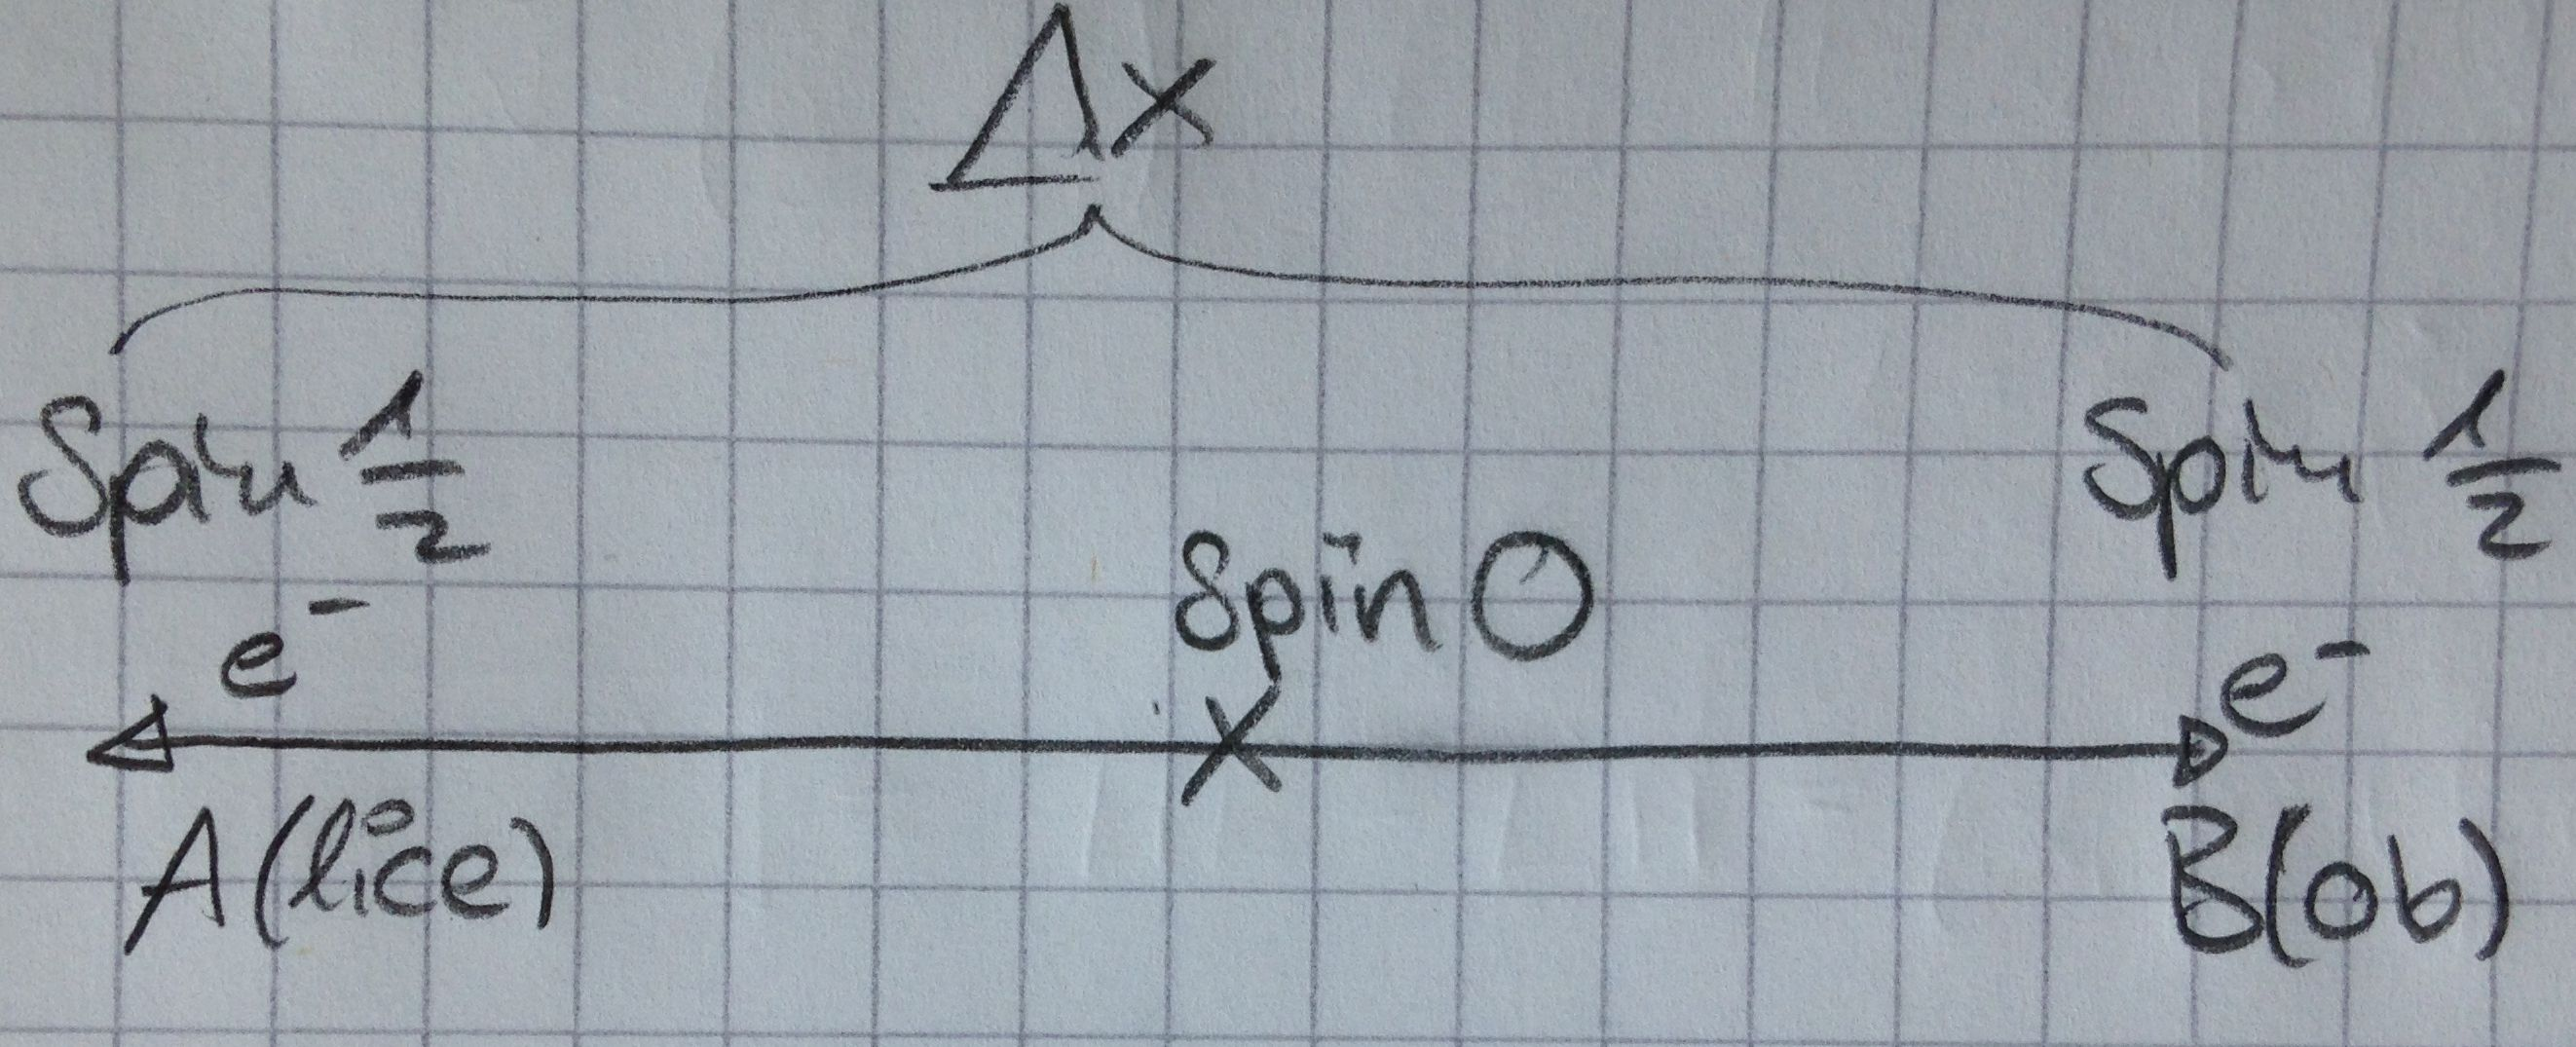
\includegraphics[width = 0.5\textwidth]{EPR_Paradox}
		\end{center}
	\end{figure}

	Drehimpulserhaltung, Singulettzustand: $S_z^{(A)} = -S_z^{(B)}$
		\begin{align*} 
			S_{z}^{(A)} &= + \frac{\hbar}{2} &
			&\Leftrightarrow &S_z^{(B)} &= -\frac{\hbar}{2} \\
			S_z^{(A)} &= -\frac{\hbar}{2}& &\Leftrightarrow &S_z^{(B)} &= + \frac{\hbar}{2} \\
			S_x^{(A)} &= + \frac{\hbar}{2}& &\Leftrightarrow &S_x^{(B)} &= - \frac{\hbar}{2} 
		\end{align*}
	Zur Zeit $t_A$ werde $S_z^{(A)} = + \frac{\hbar}{2}$ in $A$ gemessen
	
	$\Rightarrow$ Zur Zeit $t_B = t_A + \Delta t$ wird $S_z^{(B)} = -\frac{\hbar}{2}$ mit Wahrscheinlichkeit 1 in $B$  messen.
	
	(``verschränkter'' Zustand)
	
	\begin{itemize}
		\item[EPR:] Kann man den Wert einer physikalischen Größe mit Sicherheit vorhersagen, ohne ein System zu stören, dann gibt es ein ``Element der physikalischen Realität'', welches dieser Größe entspricht.
	\end{itemize}
	$B$ misst $S_z^{(B)} = -S_z^{(A)}$ zur Zeit $t_A + \Delta t$ 
	\\
	$A$ misst $S_x^{(A)} \Rightarrow B$ wird $S_x^{(B)} = -S_x^{(A)}$ messen.
	\\
	Aber $[\hat{S}_x , \hat{S}_z] \neq 0$ $S_x^{(B)}$ und $S_z^{(B)}$ sind aber nicht gleichzeitig vorhersagbar $\Rightarrow$ Es müssen weitere verborgene Variablen existieren, die mit $A$ und $B$ verknüpft sind und die Ergebnisse der Messungen festlegen.
	
	Implizit wird hierbei eine Lokalität angenommen: Wenn $\Delta t < c \Delta x$ hängen Messergebnisse am System in $A$ nur von Parametern bei $A$, Messergebnisse in $B$ nur von Parametern bei $B$ ab.